\documentclass[12pt]{article}
\usepackage{amssymb,mathrsfs, amsmath,amsfonts}
\usepackage{mathtools}
\usepackage{graphicx}
\usepackage{enumitem}
\usepackage{braket}
\graphicspath{ {./ps4-assets/}{./exercises/handwritten/ps4/ps4-assets/} }


\title{Problem Set 4}
\author{CSE 468}
\date{\today}

\begin{document}

\maketitle

\begin{enumerate}[font=\bfseries]
    \item Give the unitary matrix that describes the circuit below. Note the second gate is the controlled Z gate with $q_0$ as the control bit and $q_1$ as the target bit. Is the state at the end of this circuit entangled? Why or why not?
    \[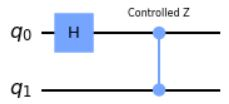
\includegraphics[scale=0.8]{cz-gate}\]
    \item Can the controlled Z gate matrix be written as the tensor product of two matrices? Prove or disprove.
    \item Question that asks what input state is entangled by CZ gate
    \item Consider standard quantum teleportation (Lecture 10). Imagine Alice has the incredible power to transmit exactly one bit to Bob instantaneously (faster than the speed of light whoa). Let's think about how this changes Bob's situation.
    \begin{enumerate}
        \item What is the probability that Bob obtains the correct state?
        \item What does Bob know about his state if Alice tells him the first qubit's value of her system?
        \item What does Bob know about his state if Alice tells him the second qubit's value of her system?
        \item If Bob only cares about getting the probabilities of his basis states right and doesn't care about the phase of his system, which qubit would he want Alice to send?
    \end{enumerate}
    \item Explain why using just a single EPR pair, Bob cannot obtain Alice's state any more than 50\% of the time without communication and ignoring phase differences.
    \item Consider the entangled state: 
    \[\ket{\psi} = \frac{1}{\sqrt{2}}(\ket{00}+\ket{11})\]
    Show that applying a general U gate to the first qubit still results in an entangled state.
    \item What is the relationship between the factorability of a 2 qubit gate and that same gate's ability to cause entanglement? (I'm not sure)
    \item Recreate the table on slide 9 in Lecture 10 (I.e. what action Bob should take for each measurement Alice could observe) if Alice and Bob used the below EPR pair to accomplish quantum teleporation.
    \[\ket{\psi} = \frac{1}{\sqrt{2}}(\ket{01}-\ket{10})\]
    \item Suppose you have the following state:
    \begin{multline} \ket{\psi} = 
        \alpha_0\ket{000} + \alpha_1\ket{001} +
                    \alpha_2\ket{010} + \alpha_3\ket{011}  \\
                    + \alpha_4\ket{100} + \alpha_5\ket{101} +
                    \alpha_6\ket{110} + \alpha_7\ket{111}
    \end{multline}
    Furthermore, suppose $|a_0|^2 = 0.5$, $|a_1|^2 = 0.25$, and $|a_5|^2 = 0.125$. Suppose you measure the first two qubits and see $00$. What is the probability of measuring 0 on the third qubit?
\end{enumerate}



\end{document}